\documentclass{article}
\usepackage[letterpaper, top=2cm, bottom =2cm, left=3cm, right=3cm,marginparwidth = 1.75cm]{geometry}
\usepackage{float}
\usepackage[brazil]{babel}
\usepackage[colorlinks = True, allcolors = Blue]{hyperref}
\usepackage[utf8]{inputenc}
\usepackage{cite}
\usepackage{natbib}
\usepackage{graphicx}
\usepackage{url}

\title{ET586 - ESTATIST PROBABILIDADE COMPUTACAO}
\author{Guilherme Cezar Menezes Siqueira}
\date{Setembro, 2023}

\begin{document}
\maketitle

\section{Introdução}
\par 
A disciplina de Estatística e Probabilidade para Computação fala sobre métodos de análise e estudo de dados, envolvendo temas como: variáveis aleatórias discretas e contínuas, análise exploratória e teste de hipótese. Ela é uma cadeira de extrema importância, visto que ela relaciona os tópicos da teoria estatística com sua aplicação na computação, assim possibilitando o estudante a interpretar certos problemas de programação a partir de uma análise amostral. É uma disciplina administrada pela professora Renata Souza e realizada, de forma obrigatória, pelos alunos do Centro de Informática da UFPE que cursam Ciência da Computação. Como base do plano de ensino da cadeira, são utilizados os livros: Noções de Probabilidade e Estatística - Marcos N. Magalhães, Antonio Carlos P. de Lima. 7ª Edição, Editora da Universidade de São Paulo e Estatística Básica - Wilton de O. Bussab, Pedro A. Morettin. 6ª Edição, Editora Saraiva.
\cite{livro_base}
\cite{livro_suplementar}
\cite{site_disciplina}

\begin{figure}[h!]
\centering
    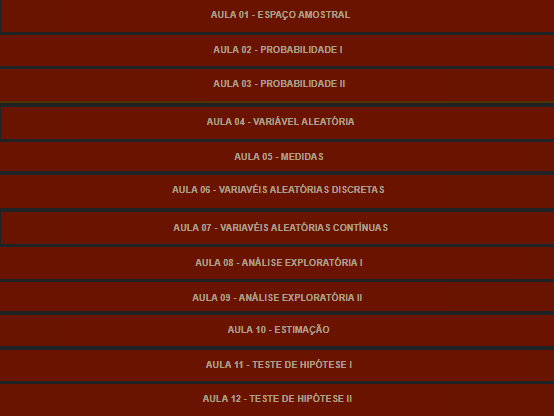
\includegraphics[width=100mm]{plano stat.png}
    \caption{Plano de Ensino ET586 - ESTATIST PROBABILIDADE COMPUTACAO. \cite{site_disciplina}}
\end{figure}

\section{Relevância}
\par
A cadeira de Estatística e Probabilidade pra Computação é de extrema relevância na composição do plano de ensino dos estudantes de Ciência da Computação, visto que ela é diretamente ligada à programação, como por exemplo nas áreas de Ciência de Dados e Aprendizado de Máquina, em que a análise amostral se torna cada vez mais crucial para a tomada de decisões. Na Ciência de Dados, o estudo estatístico é realizado a fim de extrair informações significativas para responder perguntas recorrentes e tomar conclusões no projeto em questão. Já na Inteligência Artificial, a estatística tem papel fundamental na criação uma máquina com capacidade de aprender de tomar decisões independentes, possibilitando, assim, o estudo de um grande volume de dados e a identificação de padrões não percebidos durante as análises humanas. Portanto, essa disciplina permite a abertura de diversos caminhos de desenvolvimento e cria uma base exploratória que acrescenta muito aos estudantes de tecnologia e informática do CIn.
\cite{livro_base}
\cite{livro_suplementar}

\section{Relações com outras disciplinas}
\par
A cadeira de Estatística e Probabilidade pra Computação é uma cadeira que possui um pre-requisito: MA026- CALCULO DIFERENCIAL E INTEGRAL 1, o que pode ser facilmente justificado pela presença do racícionio cálculo para o desenvolvimento de certas análises estatísticas, como por exemplo: utilizando o conceito de Integral (visto em cálculo) para o cálculo da função de densidade da probabilidade. Além de ter um pré-requisito, essa disciplina também é um pre-requisito para outras duas cadeiras: IF797- OTIMIZACAO e IF746- PROC.SIMUL.ESTOCAST.COMPUTACAO. Porém, o estudo dessa cadeira não se limita apenas para as disciplinas que ela afeta na grade curricular, pois, como vimos anteriormente na seção 2, o conteúdo dado na cadeira de estatística vai muito além do ambiente universitário, sendo um adicional imenso no desenvolvimento profissional dos estudantes do CIn.
\cite{site_curso}


\bibliographystyle{plain}
\bibliography{bibliografia.bib}

\end{document}